%-------------------------------%
%  Author: Alessandro Sciarra   %
%    Date: 17 September 2020    %
%-------------------------------%

%~~~~~~~~~~~~~~~~~~~~~~~~~~~~~~~~~~~~~~~~~~~~%
\begin{frame}[plain,noframenumbering]
    \titlepage
\end{frame}
%~~~~~~~~~~~~~~~~~~~~~~~~~~~~~~~~~~~~~~~~~~~~%
\begin{frame}[c]{Lecture format}
    \begin{center}
        \begin{tikzpicture}[every node/.style={inner xsep=0}]
            \foreach \f [count=\n from 0] in {Calendar, Time, Placeholder, Person, Newsletter}{
                \begin{scope}
                    \clip (0,-1.5*\n) circle[radius=5mm];
                    \node (A\n) at (0,-1.5*\n) {\includegraphics[width=10mm]{\f}};
                \end{scope}
            }
            \node[right = of A0] {\{26..30\}.10.2019};
            \node[right = of A1] {
                \begin{tabular}{@{}r@{\;}l}
                    Morning:   & 09:15 to 12:00 \\
                    Afternoon: & 14:15 to 17:00 \Remark[2.5mm]{I can stay more, if you wish}
                \end{tabular}
                %Morning: 09:15 to 12:00$\quad$ Afternoon: 14:15 to 17:00
            };
            \node[right = of A2] {
                \begin{tabular}{@{}r@{\;}l}
                    Morning:   & ITP, room 00.111 \Remark{Lecture with slides} \\
                    Afternoon: & ITP, room 00.111 \Remark{Exercise sheet -- I am here to help, use me}
                \end{tabular}
            };
            \node[right = of A3] {Dr. Alessandro Sciarra};
            \node[right = of A4] {sciarra@itp.uni-frankfurt.de};
        \end{tikzpicture}
    \end{center}
\end{frame}
%~~~~~~~~~~~~~~~~~~~~~~~~~~~~~~~~~~~~~~~~~~~~%
\begin{frame}{Who am I?}
    \begin{varblock}{quote}[0.68\textwidth]{Ancient popular wisdom}
        \guillemotleft{}I am not saying to be Superman, I am just saying nobody has ever seen me and Superman together in the same room.\guillemotright
    \end{varblock}
    \vspace{5mm}
    \begin{itemize}
        \item Member of the Software Development Center \\ $\to\;$ Z02 project of the CRC-TR211 collaboration
        \item A ``lattice practitioner''
        \item A dreamer who flatters himself that
              \begin{itemize}
                  \item physicists will one day \PB{properly} use the IT tools they use
                  \item IT people will teach IT to physicists and work next to them
                  \item physicists will be able to focus on physics
              \end{itemize}
        \item \PP{Not really a bash guru, but rather a self-thought bash enthusiast}
    \end{itemize}
    \begin{tikzpicture}[remember picture, overlay]
        \node[anchor=south east, inner sep=0] at (current page.south east) {
\includegraphics[height=4cm]{Superman}};
    \end{tikzpicture}
\end{frame}
%~~~~~~~~~~~~~~~~~~~~~~~~~~~~~~~~~~~~~~~~~~~~%
\begin{frame}{The mind setup of this course}
    \vspace{-3mm}
    \begin{varblock}{alerted}[0.35\textwidth]{Remember:}<3->
        \PQ{\large This is not the full story!}
    \end{varblock}
    \vspace{1mm}
    \begin{enumerate}
        \setcounter{enumi}{1}
        \item<3-> The amount of information given in this lecture is \textbf{huge}, I am aware of it
        \item<3-> You will not receive all the details (I tried to pass on the important information, though)\\
                  $\;\to\;$ be active, ask, use manuals, go beyond this lecture!
        \item<4-> Often it is hard (very hard) to clarify all details of and exceptions to rules \\
                  $\;\to\;$ experience and practice will fill the gap
        \item<4-> From rules/practical examples to abstract ideas/good practices
        \item<5-> 100\% Bash, no focus on portability or differences among \\ various shell languages \Remark{I am not at that level}\\
                  $\;\to\;$ sh, ksh, csh, tcsh, dash, zsh, fish, \ldots
        \setcounter{enumi}{0}
        \item<2-> \PS{\textbf{Relaxed atmosphere!}}\\
                  \PT{Interactive lecture: ask, ask, ask!}
    \end{enumerate}
    \begin{tikzpicture}[remember picture, overlay]
        \node[anchor=south east, visible on=<2->] (fig) at (current page.south east) {
\includegraphics[width=42mm]{Relax}};
    \end{tikzpicture}
\end{frame}
%~~~~~~~~~~~~~~~~~~~~~~~~~~~~~~~~~~~~~~~~~~~~%
\begin{frame}{What is \URL[PP]{https://www.gnu.org/software/bash/}{Bash}?}
    \begin{tikzpicture}[remember picture, overlay]
        \node[anchor=north east] (logo) at ($(current page.north east)-(3mm,3mm)$) {
\includegraphics[width=25mm]{BashLogo}};
        \node[below = 1mm of logo.north east, anchor=east, font=\tiny] {\URL{https://commons.wikimedia.org/w/index.php?curid=53428398}{Bash logo}};
    \end{tikzpicture}
    \vspace{-3mm}
    \begin{itemize}
        \item Scripting/command language
        \item Unix shell $\;\leftrightarrow\;$ command processor
        \item First release in 1989, current version v5.0 (Jan 2019) $\quad\to\;$ \URL[PS]{http://ftp.gnu.org/gnu/bash/}{download Bash}
    \end{itemize}
    \begin{varblock}{quote}[0.9\textwidth]{GNU Bash}
        Bash is the GNU Project's shell.
        Bash is the Bourne Again SHell.
        Bash is an sh-compatible shell that incorporates useful features from the Korn shell (\textnormal{ksh}) and C shell (\textnormal{csh}).
        [\ldots]
        It offers functional improvements over \textnormal{sh} for both programming and interactive use.
        In addition, most \textnormal{sh} scripts can be run by Bash without modification.
    \end{varblock}
    \uncover<2>{
        \begin{itemize}
            \item A scripting language which may get hard to read $\to$ you need some \PP{``code sense''}
            \item The effort required to a newbie is quite large $\to$ you need to practice!
            \item \ldots{}I am here to help you fill up this gap!
        \end{itemize}
    }
\end{frame}
%~~~~~~~~~~~~~~~~~~~~~~~~~~~~~~~~~~~~~~~~~~~~%
\begin{frame}{Why should I know Bash?}%{Why not a more intuitive scripting language, e.g.\ Python?}
    \vspace{-3mm}
    \begin{itemize}
        \item It is probably the shell you use (Bash is everywhere)
        \item Knowing Bash a bit more allows for better problem handling \\
              $\to\;$ e.g. delegate to Bash tasks that maybe you currently do in C/C++
        \item It is a scripting language very close to the (Unix) operative system
        \item Opportunity to make your daily work-flow more comfortable
    \end{itemize}
    %\vspace{1mm}
    \begin{varblock}{alerted}[0.64\textwidth]{}<2>
        However, \URL[PT]{http://mywiki.wooledge.org/BashWeaknesses}{Bash weaknesses} are known:\hfill
        \begin{itemize}
            \item Floating point math
            \item Lack of data structures
            \item Try/catch and Exception handling: forget them!
            \item Functions: a tricky world!
            \item \ldots
        \end{itemize}
        Knowing another scripting language (e.g.\ Python) helps!
    \end{varblock}
\end{frame}
%~~~~~~~~~~~~~~~~~~~~~~~~~~~~~~~~~~~~~~~~~~~~%
\begin{frame}{What to expect from the lecture?}
    \vspace{-3mm}
    \begin{varblock}{quote}[1.02\textwidth]{My point of view as physicist}
        The way you program today is better than it was yesterday and probably worse than it will be tomorrow!
        Bash has some kind of subjective corners where you will have to choose your way.
        Have a good reason to do things the way you do them.
        It will happen that you will change mind and consequently your approach to the same problem.
        Again and over again, it is normal.
        Do not hesitate in doing so.
        To change mind and approach means to evolve and to become a better programmer.
    \end{varblock}
    \begin{itemize}
        \item This is especially important as physicist
        \item Knowing all details and tweaks of Bash is probably not your goal \\
              $\;\to\;$ nor is it probably needed in your daily work
        \item \PT{Having an overview} is, instead, very important (e.g.\ to \PT{decide when to use Bash})
        \item As soon as something smells odd, it is important \PT{to be able to have a detailed look}
    \end{itemize}
    \begin{varblock}{}[0.8\textwidth]{}%Can I switch this integral with this sum?}
        %Usually a physicist assumes it is possible and goes back as soon as something starts looking odd\ldots
        \PB{$\displaystyle\sum\int(\ldots)=\int\sum(\ldots)$ until something starts looking odd}
    \end{varblock}
    
\end{frame}
%~~~~~~~~~~~~~~~~~~~~~~~~~~~~~~~~~~~~~~~~~~~~%
\begin{frame}{References for future use}
    \vspace{-4mm}
    \PB{\underline{About Bash world}:}
    \begin{itemize}
        \item[] \URL{https://www.gnu.org/software/bash/manual/}{Bash official manual}
        \item[] \URL{http://manpages.ubuntu.com/manpages/bionic/man7/bash-builtins.7.html}{List of Bash builtins with descriptions}
        \item[] \URL{http://mywiki.wooledge.org/BashFAQ/061}{Notable changes in released bash versions}\PB{\Remark{More extensive list \URL[PB]{http://wiki.bash-hackers.org/scripting/bashchanges}{also available}}}
        \item[] \URL{https://devhints.io/bash}{A nice Bash cheatsheet}
        \item[] \URL{https://google.github.io/styleguide/shellguide.html}{Google Shell Style Guide}
        \item[] \URL{https://github.com/mietek/bashmenot}{A (sadly not maintained) Bash library}\PB{\Remark{Clone from Github to use it, reference website is unfortunately down}}
        \item[] \URL{https://explainshell.com/}{An online help to get relevant manual pages of a given command}
    \end{itemize}
    \vspace{1mm}
    \PB{\underline{Didactical material}:}
    \begin{itemize}
        \item[] \URL{http://tldp.org/LDP/Bash-Beginners-Guide/html/}{Bash Beginners Guide}\PB{\Remark{A nice, from-zero tutorial}} \tikzmark{TutorialBegin}
        \item[] \URL{https://www.shellscript.sh/}{Shell scripting tutorial}\PB{\Remark{Nice tutorial, but not only Bash}}
        \item[] \URL[PS]{http://mywiki.wooledge.org/BashGuide}{Bash Guide}\PB{\Remark{Very precise guide, not completely from zero, though -- AKA Greg's Wiki}} \tikzmark{TutorialEnd}
        \item[] \URL{https://github.com/AxelKrypton/Bash_lecture_2020}{All material \tikzmark{MeOnGitHub}of this lecture}
    \end{itemize}
    \begin{tikzpicture}[remember picture, overlay]
        \draw[very thick, decorate, decoration={brace,amplitude=6pt}] (TutorialBegin -| TutorialEnd) ++(5mm,1mm) -- ($(TutorialEnd)+(5mm,-1mm)$) 
              node[midway, right=3mm, text width=25mm, font=\small, align=center, text=PP] {Material used to prepare this lecture};
        \path[to] (MeOnGitHub) ++(0,-2mm) edge[out=270, in=180] node[pos=1, anchor=west] {My GitHub page \hspace{1mm}\raisebox{-1.3mm}{
\includegraphics[width=5mm]{AxelKrypton}}} ++(20mm, -4mm);
        \node[anchor=north, inner ysep=3mm] (book) at ($(current page.north)!0.5!(current page.north east)$) {
\includegraphics[width=16mm]{Cookbook}};
        \node[right = 1mm of book, inner ysep=3mm] {
\includegraphics[width=16mm]{LearningBash}};
        \path[from] (TutorialEnd) ++(-0mm,-1mm) edge[out=330, in=180] node[pos=1, right=2pt, font=\scriptsize, text=PS, text width=20mm, align=center] {Main reference for preparing this course} ++(12mm, -6mm);
    \end{tikzpicture}
\end{frame}
%~~~~~~~~~~~~~~~~~~~~~~~~~~~~~~~~~~~~~~~~~~~~%
\begin{frame}{What will we explore?}
    \colorlet{Monday}{PT}
    \colorlet{Tuesday}{PS}
    \colorlet{Wednesday}{Crimson}
    \colorlet{Thursday}{Teal}
    \colorlet{Friday}{RoyalBlue}
    \vspace{-5mm}
    \begin{multicols}{2}
        \begin{enumerate}
            \item \tc<2>{Monday}{Inception and philosophy}
            \item \tc<2>{Monday}{Commands and arguments}
            \item \tc<2>{Monday}{Strings and types of commands}
            \item \tc<2>{Monday}{Quoting and special characters}
            \item \tc<2>{Monday}{Variables and special parameters}
            \item \tc<2>{Monday}{Shell expansion and word splitting}
            \item \tc<2>{Monday}{Patterns}
            \item \tc<2>{Tuesday}{Flow control}
            \item \tc<2>{Tuesday}{Colours and terminal commands}
            \item \tc<2>{Tuesday}{Namerefs and indirect expansion}
            \item \tc<2>{Tuesday}{Arrays and associative arrays}
            \item \tc<2>{Tuesday}{Input and output}
            \item \tc<2>{Tuesday}{Shell options and GNU Coreutils}
            \item \tc<2>{Wednesday}{File descriptors and redirection}
            \item \tc<2>{Wednesday}{Compound commands}
            \item \tc<2>{Wednesday}{Functions}
            \item \tc<2>{Wednesday}{Script autocompletion and GNU Redline}
            \item \tc<2>{Thursday}{Asynchronous commands}
            \item \tc<2>{Thursday}{Traps}
            \item \tc<2>{Thursday}{Error handling}
            \item \tc<2>{Thursday}{Sed}
            \item \tc<2>{Friday}{Awk}
            \item \tc<2>{Friday}{Some good practices and useful tools}
            \item \tc<2>{Friday}{Bash in real life}
            \item \tc<2>{Friday}{An interactive summary}
            \item \tc<2>{Friday}{What to do now?}
        \end{enumerate}
    \end{multicols}
    \begin{tikzpicture}[remember picture, overlay, every label/.append style={label distance=-2pt, font=\tiny}, scope on=<2>]
        \foreach \d/\n [count=\i] in {Monday/26, Tuesday/27, Wednesday/28, Thursday/29, Friday/30}{
            \node[anchor=north, draw, rounded corners=1pt, label={[\d]90:\d}, inner ysep=1mm, inner xsep=2mm, text=\d, draw=\d, fill=\d!5] (Mon) at ($(current page.north)+(\i cm,-5mm)$) {\n\vphantom{2367890}};
        }
    \end{tikzpicture}
\end{frame}
%~~~~~~~~~~~~~~~~~~~~~~~~~~~~~~~~~~~~~~~~~~~~%
\begin{frame}[fragile]{A slide about notation}
    \vspace{-5mm}
    \begin{varblock*}{quote}[0.72\textwidth]{Slides notation}
        \normalfont
        \begin{itemize}
            \setlength{\itemindent}{-1mm}
            \item Slides are (too) full of text for a later reading!
            \item Many examples to immediately show you how rules apply
            \item In Bash code, syntax highlighted to help recognise the elements
            \item Prompt commands are always preceded by a dollar sign 
                  \begin{lstlisting}[style=MyBash, numbers=none, aboveskip=2mm, xleftmargin=1mm, xrightmargin=12mm]
                      $ ls
                  \end{lstlisting}
                  \Remark{When the \texttt{\$} is absent, the code refers to a script or it is pseudo-code}
        \end{itemize}
    \end{varblock*}
    \colorlet{Study}{DarkGreen}
    \colorlet{Instructive}{DodgerBlue}
    \colorlet{Inspirational}{OrangeRed}
    \colorlet{Technical}{black}
    \begin{varblock*}{alert}[0.57\textwidth]{Exercise colour notation}
        \begin{itemize}
            \setlength{\itemindent}{-1mm}
            \item \tc{Study}{Review the morning lecture}
            \item \tc{Instructive}{Focusing on and playing with a Bash feature}
            \item \tc{Inspirational}{Inspirational for real life}
            \item \tc{Technical}{Technical}
        \end{itemize}
    \end{varblock*}
    \FrameRemark{This note usually provides further (advanced) information. Links here are worth the read.}
\end{frame}
%~~~~~~~~~~~~~~~~~~~~~~~~~~~~~~~~~~~~~~~~~~~~%
\begin{frame}{Bonus track\uncover<2>{: Iceland}}{\uncover<2>{The magic of an incredible island}}
    \begin{tikzpicture}[remember picture, overlay, scope on=<2>]
        \node[inner sep=0pt] (plan) at ($(current page.center)-(0,6mm)$) {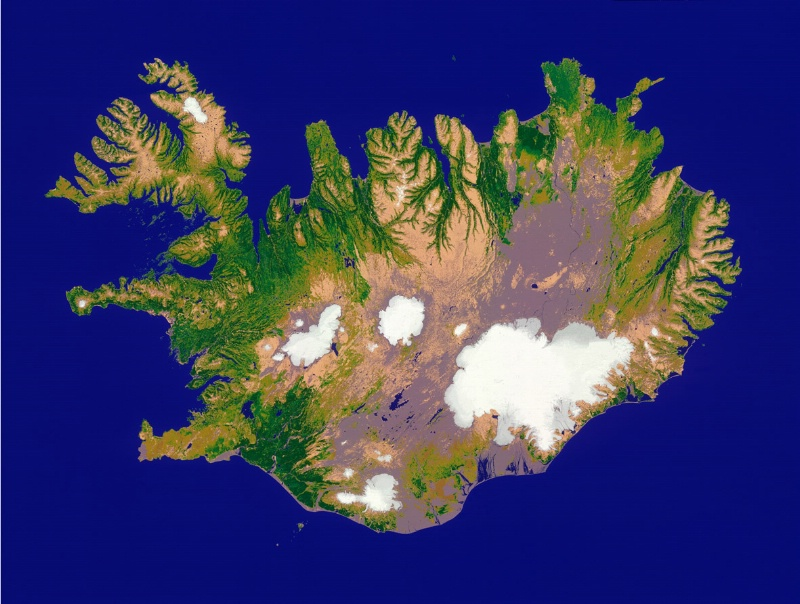
\includegraphics[width=0.8\textwidth, clip, trim=1mm 0 0 0]{Map2}};
        \begin{scope}[x={($ (plan.south east) - (plan.south west) $ )},y={( $ (plan.north west) - (plan.south west)$ )}, shift={(plan.south west)}]
            %\draw[help lines,xstep=.1,ystep=.1] (0,0) grid (1,1);
            \node[anchor=south, inner sep=0] at (0.175,0.280) {
\includegraphics[width=3mm]{Pin}};
            \node[anchor=south, inner sep=0] at (0.180,0.238) {
\includegraphics[width=3mm]{Pin}};
            \node[anchor=south, inner sep=0] at (0.255,0.260) {
\includegraphics[width=3mm]{Pin}};
            \node[anchor=south, inner sep=0] at (0.235,0.240) {
\includegraphics[width=3mm]{Pin}};
            \node[anchor=south, inner sep=0] at (0.240,0.310) {
\includegraphics[width=3mm]{Pin}};
            \node[anchor=south, inner sep=0] at (0.320,0.350) {
\includegraphics[width=3mm]{Pin}};
            \node[anchor=south, inner sep=0] at (0.310,0.290) {
\includegraphics[width=3mm]{Pin}};
            \node[anchor=south, inner sep=0] at (0.335,0.270) {
\includegraphics[width=3mm]{Pin}};
            \node[anchor=south, inner sep=0] at (0.370,0.355) {
\includegraphics[width=3mm]{Pin}};
            \node[anchor=south, inner sep=0] at (0.400,0.155) {
\includegraphics[width=3mm]{Pin}};
            \node[anchor=south, inner sep=0] at (0.450,0.140) {
\includegraphics[width=3mm]{Pin}};
            \node[anchor=south, inner sep=0] at (0.480,0.120) {
\includegraphics[width=3mm]{Pin}};
            \node[anchor=south, inner sep=0] at (0.655,0.295) {
\includegraphics[width=3mm]{Pin}};
            \node[anchor=south, inner sep=0] at (0.705,0.265) {
\includegraphics[width=3mm]{Pin}};
            \node[anchor=south, inner sep=0] at (0.730,0.340) {
\includegraphics[width=3mm]{Pin}};
            \node[anchor=south, inner sep=0] at (0.735,0.305) {
\includegraphics[width=3mm]{Pin}};
            \node[anchor=south, inner sep=0] at (0.810,0.400) {
\includegraphics[width=3mm]{Pin}};
        \end{scope}
        \node[below = 3mm of plan.south east, anchor=east, font=\tiny] {{\raisebox{-2mm}{\Large\textcopyright}} Photos throughout the lecture: All rights are reserved};
    \end{tikzpicture}
\end{frame}
%~~~~~~~~~~~~~~~~~~~~~~~~~~~~~~~~~~~~~~~~~~~~%
\begin{frame}{A short but intense journey}{A few more recommendations}
    \vspace{-3mm}
    \begin{itemize}
        \item I am aware that you will receive a lot (really a lot) of information
        \item Do not hesitate to ask!
        \item Put effort into the exercises
        \item The more active you are the more information will stay in your memory for your daily work
    \end{itemize}
    \vspace{5mm}
    {\large\PP{What do I expect?}}
    \begin{itemize}[<2->]
        \item You will also learn general coding principles, which are independent of the language \\
              {\small$\;\to\;$ \URL[PP]{https://crc-tr211.org/seminar_slides_GU/2019.06.03.sciarra.pdf}{Clean code talk given on 03.06.2019}}
        \item You enjoy the journey! \Remark{\ldots{}at least discovering Iceland\ldots}
        \item \PS{You give me feedback at the end of the lecture!}
    \end{itemize}
    \vfill\hfill\uncover<3>{\LARGE\PT{Are you ready?}\hspace{3mm}}
\end{frame}
%~~~~~~~~~~~~~~~~~~~~~~~~~~~~~~~~~~~~~~~~~~~~%